\documentclass[../main.tex]{subfiles}
\begin{document}
\subsection{Pre-Calculus}
\begin{itemize}
\item Exercise: $S:x^2+y^2+z^2=16$\\
Lies above $xy$-plain and inside $x^2+y^2\leq 4$
\begin{itemize}
\item Parameterize S
\begin{equation}
    z = \sqrt{16 - x^2 - y^2}
\end{equation}
Let $x = u$, $y=v$
\begin{equation}
r(u,v) = (u,v,\sqrt{16-u^2-v^2},~\text{where }u^2+v^2 \leq 4
\end{equation}
Note: $x^2+y^2=16 \Rightarrow r(t) = (4\cos(t), 4\sin (t))$
\item Use cylindrical coordinates
\begin{equation}
x = r\cos \theta,~
y=r\sin \theta ~
z = f(r,\theta) = \sqrt{16 - r^2}
\end{equation}
最後寫得:
\begin{equation}
\mathbf{r}(r,\theta) = (r\cos\theta, r\sin\theta, \sqrt{16-r^2} )
\end{equation}
Where $r \in[0,1],~ \theta \in [0,2\pi]$
\item Spherical Coordinate
\begin{equation}
x=r\sin\phi\cos\theta,~
y=r\sin\phi\sin\theta,~
z= r\cos\phi
\end{equation}
Remark $x^2+y^2+z^2 = r^2$
\begin{equation}
x = 4\sin\phi\cos\theta,~
y = 4\sin\phi\sin\theta,~
z = 4 \cos\phi
\end{equation}
最後得到:
\begin{equation}
\mathbf{r}(\phi,\theta) = \left( \underline{\hspace{1cm}}, \underline{\hspace{1cm}}, \underline{\hspace{1cm}}
\right),~\text{where }\theta \in [0,2\pi], ~\phi\in[0,\frac{\pi}{6}] 
\end{equation}
注意範圍限制:
\begin{equation}
    x^2 + y^2 = 16 \sin^2 \phi \leq 4,~
    \sin^2\phi \leq \frac{y}{4} \implies \phi \leq \frac{\pi}{6}
\end{equation}
\end{itemize}
\item Excercise 2
\begin{enumerate}
\item  $x^2+y^2+z^2=2z$ sphere, lies inside $z=x^2+y^2$\\
Proof: 
\begin{equation}
x^2+y^2+(z-1)^2=1,~\begin{cases}
\text{center } (0,0,1) \\
\text{radius} = 1
\end{cases}
\end{equation}
Use cylindrical:
\begin{equation}
\begin{cases}
x = r\cos \theta\\
y = r\sin\theta
\end{cases}\implies z = r^2
\end{equation}
Note:
\begin{equation}
x^2+y^2 +z^2 = 2z,~x^2+y^2 = z
\end{equation}
View quadratic of $z$
\begin{equation}
r^2 + z^2 = 2z \implies z = 1 \pm \sqrt{1-r^2}
\end{equation}
Only take positive since lies inside $z=x^2+y^2$\\
所以
\begin{equation}
\mathbf{r}(r,\theta) = (r\cos\theta,~r\sin\theta,~1+\sqrt{1-r^2}),~r\in[0,1],~\theta\in[0,2\pi]
\end{equation}
\item Cone: $z = \sqrt{3(x^2+y^2)}$, lies below
$z = 2+x$\\
Proof:
\begin{equation}
\begin{cases}
  x = r\cos\theta,~ y = r\sin\theta \implies
  z = \sqrt{3r^2} = \sqrt{3}r
\end{cases}
\end{equation}
Because lies below $z = 2+z$
\begin{equation}
\sqrt{3} r \leq 2 + r\cos\theta
\end{equation}
Note:
\begin{equation}
(\sqrt{3}-\cos\theta)r \leq 2 \implies r\leq\frac{2}{\sqrt{3}-\cos\theta}
\end{equation}
Ans:
\begin{equation}
\mathbf{r}(r,\theta) = \left(
\underline{\hspace{1cm}},\underline{\hspace{1cm}}, \sqrt{3}r
\right), \text{where }\theta \in[0,2\pi],r\in\left[
0, \frac{2}{\sqrt{3}-\cos\theta}
\right]
\end{equation}
\end{enumerate}
\item Excercise 3:
\begin{enumerate}
\item $S_1: x^2 + y^2 + z^2 =1$, lies below $z=\frac{1}{2}$\\
Proof:
\begin{equation}
x = \sin\phi\cos\theta,~
y = \sin\phi\sin\theta,~
z = \cos\phi
\end{equation}
We have $\cos\phi \leq \frac{1}{2} $
\begin{equation}
\phi \in \left[
\frac{\pi}{3},~\pi
\right],~\theta\in[0,2\pi]
\end{equation}
\item $S_2: x^2+y^2+(z-1)^2 = 1$ lies above $z=\frac{1}{2}$\\
Proof:
\begin{equation}
x = \sin\phi\cos\theta,~y = \sin\phi\sin\theta,~ z= \cos\phi+1
\end{equation}
We have:
\begin{equation}
\cos\phi +1 \leq \frac{1}{2} \implies \cos\phi \leq -\frac{1}{2} 
\implies \phi \in\left[
0, \frac{2\pi}{3}
\right] 
\end{equation}
\end{enumerate}
\item Excercise 4\\
$S_1: x^2+4y^2+4z^2 = 4,~x\leq 0$
\begin{equation}
 \implies \frac{x^2}{4}+y^2+z^2 = 1:~\text{semi-axis } 2,1,1
\end{equation}
得到:
\begin{equation}
x = 2\cos\phi
y = \sin\phi\cos\theta
z = \sin\phi\sin\theta
\end{equation}
所以
\begin{equation}
2\cos\phi \leq 0 \implies \cos\phi \leq 0 \implies \frac{\pi}{2}\leq \phi \leq \pi
\end{equation}
$S_2: x = 4-4y^2-4z^2,~x\geq 0$
\begin{equation}
y = r\cos\theta,~z=r\sin\theta \implies x=4-4r^2 \geq 0 \implies r\in[0,1], \theta \in [0,2\pi]
\end{equation}
\end{itemize}
\subsection{Convergence of Sequences}
Def:
\begin{enumerate}
  \item $A$ sequence $x_n(n\in \mathbb{N})$ in a set $S$ is a map
  \begin{equation}
  \mathbb N \xrightarrow{x_1} S, n \mapsto x_n
  \end{equation}
\item A subsequence $x_{n_k}$ of a sequence $x_n$ is given by compositon
\begin{equation}
N \xrightarrow{n_1} \mathbb N \xrightarrow{n_2} S, k \mapsto n_k \mapsto x_{n_k}
\end{equation}
of $x$, with a strictly meaning way $\mathbb N \to \mathbb N, k \mapsto n_k$.
\item Sphere that $S \subseteq R^N$, we say that a sequence of $x_n(n\in \mathbb{N})$ on $S$ converges to a point $p\in R^k$ if
$\forall \varepsilon > 0, \exists N \in \mathbb{N}$ such that
$\forall n \in \mathbb{N},~(x_n\in B(p)), n \geq N \implies \left|x_n - p\right| < \varepsilon$.\\
example for sequence that does not converge:
\begin{itemize}
  \item $x_n \in (-1)^n (n\in \mathbb{N})$ in $\mathbb{R}$.\\
  Diverges, but has convergent subsequences
\end{itemize}
Lemma: How close are closed subsets?
\begin{itemize}
  \item For $S \subseteq R^k$
  \begin{equation}
  \boxed{S \subseteq \text{closed} R^k \Leftrightarrow \forall \text{seq} x_n(n\in \mathbb{N}) \text{ in } S,
   x_n \to P \implies p \in S
  }
  \end{equation}
  Proof:\\
  Proof by contradiction.\\
  Suppose that $\exists$ seq $x_n(n \in \mathbb{N})$ in $S$ such that
  $x_n \to P$ as $n \to \infty$ for some $p$,\\
  but $p\notin S$, then $\implies \exists \varepsilon >0$ such that\\
  $B_\varepsilon(p) \subseteq R^n / S$ (span in $R^n$)\\
  Since $x_n \to p$ as $n \to \infty$, $\exists N \in \mathbb{N}$, $n \geq N \implies x_n \in B_\varepsilon(p) = \emptyset$,
  which contradicts the definition of $B_\varepsilon(p)$.\\
  Proof by contradiction.\\
  Suppose that $S$ is not closed, then $R^k / S$ is not open in $\mathbb{R}^k$, 
  $\implies \exists p \in \mathbb{R}^k / S, \forall r> 0, B_r(p) \nsubseteq R^{k} / S$\\
  ($\implies B_r(p) \cap S \neq \emptyset$)
\end{itemize}
\item The Weirstrab theorem:\\
Every subsequence $x_n(n \in \mathbb{N})$ in a bounded (and closed) subset $S$ of $\mathbb{R}^k$ 
has a convergent subsequence. (When limit lies in $S$)\\
Proof:\\
$R^2$:
\begin{figure}[H]
  \centering
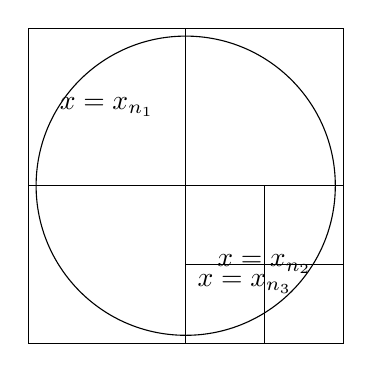
\begin{tikzpicture}
  \draw (0,0) rectangle (4,4);
  \draw (2,0) -- (2,4);
  \draw (0,2) -- (4,2);
  \draw (2,2) circle (1.9);
  \node at (1,3) {$x=x_{n_1}$};
  \node at (3,1) {$x=x_{n_2}$};
  \draw (3,0) -- (3,2);
  \draw (2,1) -- (4,1);
  \node at (2.75,0.75) {$x=x_{n_3}$};
\end{tikzpicture}
\end{figure}
Suppose that the right bottom corner has $x_n$ for infinetely index $n$
\item Def (uniform continuity):\\
A map $S \xrightarrow{f} R^l, S \subseteq \mathbb{R}^k$ is sait to be uniformly continuous if
\begin{equation}
\forall \delta > 0, \forall y \in S, \forall x \in S \exists \varepsilon > 0
\end{equation}
and
\begin{equation}
\left| x - y \right| < \delta \implies \left|
f(x) - f(y)
\right| < \varepsilon
\end{equation}
continuous
\begin{equation}
\forall \varepsilon S, \exists \delta > 0, \forall x \in S
\end{equation}
and
\begin{equation}
\left| x- y\right| < \delta \implies \left| f(x) -f(y) \right| < \varepsilon, \lim_{x\to y} f(x) = f(y)
\end{equation}
for example:
\begin{equation}
f(x) = \frac{1}{x},~ (0, \infty) \xrightarrow{f} \mathbb{R}, x \mapsto \frac{1}{x}
\end{equation}
\begin{figure}[H]
  \centering
\begin{tikzpicture}
\end{tikzpicture}
\end{figure}
then
\begin{equation}
\delta = y + \frac{1}{\frac{1}{y} + \varepsilon}
\end{equation}
Is continuous but not uniformly continuous.
\item Theorem:\\
Uniform continuity on bounded and closed subset in $\mathbb{R}^k$\\
Every contridition map $S \xrightarrow{f} R^l, S \subseteq \mathbb{R}^k$ on a bold and closed $S$ in $\mathbb{R}^k$ 
is uniformly continuous.\\
Proof:\\
By contradiction.\\
Suppose that
\begin{equation}
\exists \varepsilon > 0 \forall \delta >0 \exists y \in S \forall x \in S
\end{equation}
such that
\begin{equation}
\left| x - y \right| < \delta
\end{equation}
and
\begin{equation}
\left| f(x) - f(y) \right| \geq \varepsilon
\end{equation}
In particular, for every $n \in \mathbb{N}$, there are $x_n$ and $y_n$ $\in S$ such that
\begin{equation}
\left| x_n - y_n \right| < \frac{1}{n}
\end{equation}
and
\begin{equation}
\left| f(x_n) - f(y_n) \right| \geq \varepsilon.
\end{equation}
By the Wierstrab theorem, there $\exists$ subsequence $x_{n_k}$($k\in \mathbb{N}$) of $x_n(n \in \mathbb{N})$ which converges to a point $p$ .
\begin{equation}
\left| x_{n_k} - p \right| \leq \left|
x_{}{n_k} - y_{n_k}\right| + \left| y_{n_k} - p \right|
\end{equation}
Therefore:
\begin{equation}
\varepsilon \leq \left| f(x_{n_k}) - f(y_{n_k}) \right| \leq \left| f(x_{n_k}) - f(p) \right| + \left| f(p) - f(y_{n_k}) \right|
\end{equation}
\item Parametrized integrals\\
Examples:
\begin{equation}
\phi(u) = \int_a^b g(u,t)
\end{equation}
Properties\\
Let $[a,b] \times \Omega \xleftarrow{g} \mathbb{R}$ ( $\Omega \subseteq \mathbb{R}$ is open) 
be a map, and $u_0 \in \Omega$.\\
Suppose that
\begin{enumerate}
  \item $\forall u \in \Omega,~[a,b]\xleftarrow{g(\cdot, u)} \mathbb{R}$ is continuous
  \item $\forall t \in [a,b]$, $g$ is continuous at $(t_0,u_0)$
\end{enumerate}
Then $\phi(u) = \int_a^b g(t,u)dt$ is continuous at $u_0$.\\
Proo
Consider
\begin{equation}
\left| \phi(u) - \phi(u_0) \right| = \left| \int_a^b g(t,u) - g(t,u_0)dt \right| \leq \int_a^b
\left|
g(t,u) - g(t,u_0)
\right|
\end{equation}
Claim $\forall \varepsilon > 0 \exists \delta > 0 \forall t \in [a,b]\forall u \in \Omega$
\begin{equation}
\left| u - u_0 \right| < \delta \implies \left| g(t,u) - g(t,u_0) \right| < \varepsilon  
\end{equation}
Suppose that
\begin{equation}
\exists \varepsilon >0 \forall \delta > 0 \exists t \in [a,b] \exists u \in \Omega
\end{equation}
Such that $\left| u - u_0 \right| < \delta$ and $\left| g(t,u) - g(t,u_0) \right| \geq \varepsilon$\\
In particular, for every $n \in \mathbb{N}$, there are $t_0 \in [a,b]$ and $u_n \in \Omega$ \\
such that $\left| u_n - u_0 \right| < \frac{1}{n}$ and 
$\left| g(t_0,u_n) - g(t_0,u_0) \right| \geq \varepsilon$.\\
Since $[a,b] \subseteq \mathbb{R}$ and closed by the $W$ theorem, $\exists$ convergent subsequence $t_{n_k}(k\in \mathbb{N})$
of $t_n(n \in \mathbb{N})$ say, $t_{n_k} \mapsto t_0$ as $k \to \infty$.\\
Then $(t_{n_k},u_{n_k}) \mapsto (t_0,u_0)$ .\\
By (2), $f(t_{n_k},u_{n_k}) \mapsto f(t_0,u_0)$ as $k \to \infty$, which contradicts the definition of $\varepsilon$.\\
By the claim $\forall \varepsilon > 0 \exists \delta > 0 \forall u \in \Omega, \forall t \in [a,b]$
\begin{equation}
\left| u - u_0 \right| < \delta \implies \left| g(t,u) - g(t,u_0) \right| <
\frac{\varepsilon}{b-a} \implies \left|\phi(u) - \phi(u_0) \right| < \varepsilon
\end{equation}
Then
\begin{itemize}
  \item Then  $\phi(u) = \int_a^b g(t,u)dt$ is contiunous at $u_0$.
  \item If, furthermore, $\frac{\partial g}{\partial u_0}(t,u)$ exists for every $(t,u)$ and 
  $\frac{\partial g}{\partial u_0}$ is contiunous at $(t_0,u_0)$ for every $t_0 \in [a,b]$,
  and $\frac{\partial g}{\partial u_0}(\cdot, u)$ is continuous at $[a,b]$ for every $u\in \Omega$,
  then $\frac{\partial \phi}{\partial u_0}(u) = \int_a^b \frac{\partial g}{\partial u_0}(t,u)dt$\\
  Proof:
  \begin{align}
  \left| \frac{\phi(u_0+h e_i) - \phi (u_0)}{h} - \int_a^b \frac{\partial g}{\partial u_0}(t,u_0)dt \right|
   &= \left|
    \int_a^b \frac{g(t,u_0 + h e_i) - g(t,u_0)}{h} - \frac{\partial g}{\partial u_0}(t,u_0)dt \right| \nonumber\\
    &\leq \int_a^b \left|
    \frac{\partial g}{\partial u_i}(t,u_0+\tilde{h}(t)e_i) - \frac{\partial g}{\partial u_0}(t,u_0)
    \right| \nonumber\\
    &\leq \int_a^b \frac{\varepsilon}{b-a} dt \nonumber\\
    &= \varepsilon
  \end{align}
  for some $\tilde{h}(t)$ between $0$ and $h$ $\to$ 0 as $h \to 0$.\\
  Applying the previous claim to $\frac{\partial g}{\partial u_0}$ shows that for any given $\varepsilon > 0$,
  there exists some $\delta > 0$ such that whenever $u< \Omega$ satisfies $\left| u - u_0 \right| < \delta$,
   we have 
   \begin{equation}
   \left| \frac{\partial g}{\partial t}(t,u) - \frac{\partial g}{\partial t}(t,u_0) \right| < \frac{\varepsilon}{b-a}
   \end{equation}
   for every $t \in [a,b]$.\\
   Therefore, for every $h$ with $\left| h \right| < \delta$, we have
   \begin{align}
  \left| \frac{\phi(u_0+h e_i) - \phi (u_0)}{h} - \int_a^b \frac{\partial g}{\partial u_0}(t,u_0)dt \right|
   &= \left|
    \int_a^b \frac{g(t,u_0 + h e_i) - g(t,u_0)}{h} - \frac{\partial g}{\partial u_0}(t,u_0)dt \right| \nonumber\\
    &\leq \int_a^b \left|
    \frac{\partial g}{\partial u_i}(t,u_0+\tilde{h}(t)e_i) - \frac{\partial g}{\partial u_0}(t,u_0)
    \right| \nonumber\\
    &\leq \int_a^b \frac{\varepsilon}{b-a} dt \nonumber\\
    &= \varepsilon
  \end{align}
\end{itemize}
\item Arc length of parameterized curves:\\
If $\Delta'$ is finer than $\Delta$ (i.e. $\Delta' \supseteq \Delta$), then $\Lambda(y,\Delta') \geq \Lambda(y,\Delta)$.\\
Given a map $[a,b] \xrightarrow{\gamma} \mathbb{R}^n$, and subdivision $\Delta$ of $[a,b]$, say, $\Delta = \left\{
  t_0^\Delta, t_1^\Delta, \cdots, t_{k(\Delta)}^\Delta
\right\}$ with $a= t_0^\Delta < t_1^\Delta < \cdots < t_{k(\Delta)}^\Delta = b$,\\
we let
\begin{enumerate}
  \item $\Lambda(\gamma, \Delta) = \sum_{i=1}^{k(\Delta)} \left\| \gamma(t_i^\Delta) - \gamma(t_{i-1}^\Delta) \right\|$
  \item $\Lambda(\gamma) := \text{sup} \left\{
    \Lambda(\gamma, \Delta) | \Delta : \text{a subdivision of } [a,b]
  \right\}$
\end{enumerate}
We say that $\gamma$ is rectifiable if $\Lambda(\gamma) < \infty$.
\item Example:
\begin{equation}
  U = \mathbb{R}^2 / \left\{(0,0)\right\} \xrightarrow{F} \mathbb{R}^2, (x,y) \mapsto \left<
    \frac{-y}{x^2+y^2}, \frac{x}{x^2+y^2}
  \right>
\end{equation}
and
\begin{equation}
  \gamma(t)= (R(t)\cos\theta(t), R(t)\sin\theta(t)), a\leq t \leq b
\end{equation}
with $R(\cdot), \theta(\cdot) : C^1$\\
Solve:
\begin{align}
\int_\gamma F \cdot dr &= \int_a^b F(\gamma(t)) \cdot \gamma'(t) dt \nonumber\\
&= \int_a^b \left<
  \frac{-R(t)\sin\theta(t)}{R(t)^2}, \frac{R(t)\cos\theta(t)}{R(t)^2}
\right> \cdot \left(R'(t)\left<\cos\theta(t), i\sin\theta(t)
\right>+ R(t)\left<
-\sin\theta w, \cos\theta(t)
\right>\right) \nonumber\\
&=\int_a^b \theta'(t)dt = \theta(b) - \theta(a)
\end{align}
\item Reparameterization\\
Properties For any $F: U \to \mathbb{R}$  is continuous\\
We have
\begin{equation}
\int_{\gamma} F \cdot dr = \int_{\gamma = \sigma} F\cdot dr
\end{equation}
Proof:
\begin{align}
\int_\gamma F \cdot dr &= \int_a^b F(\gamma(t))\cdot \gamma'(t) dt \nonumber\\
&=\int_\alpha^\beta F(\gamma(\sigma(\tau))\cdot \gamma'(\sigma(\tau))\sigma'(\tau) d\tau \nonumber\\
&=\int_\alpha^\beta F(\gamma\cdot \sigma) (\tau)(\gamma\cdot \sigma)'(\tau) d\tau \nonumber\\
&= \int_{\gamma\cdot \sigma}^\alpha F\cdot dr
\end{align}
\item Remark (about putting several curves together)
\begin{figure}[H]
\centering
\begin{tikzpicture}[
  scale=1.0,
  >=Latex,
  curve/.style={thick, decorate,
    decoration={snake, amplitude=0.7mm, segment length=7mm}},
  axis/.style={thin},
  lab/.style={font=\small}
]
    \draw[axis] (-4.6,1.8) -- (-3.0,1.8);
\draw[axis] (-4.6,1.7) -- (-4.6,1.9);
\draw[axis] (-3.0,1.7) -- (-3.0,1.9);
\node[lab] at (-4.6,1.45) {$a_1$};
\node[lab] at (-3.0,1.45) {$b_1$};
\node[lab] at (-3.8,2.08) {$\gamma_1$};

% curve gamma_1 in U
\draw[curve, red!70!black]
  (-1.8,2.0)
  .. controls (-1.1,2.8) and (-0.5,2.5) .. (-0.1,1.9)
  .. controls (0.2,1.4) and (0.8,1.4) .. (1.1,1.9);

% small interval gamma_2
\draw[axis] (-4.6,0.35) -- (-3.0,0.35);
\draw[axis] (-4.6,0.25) -- (-4.6,0.45);
\draw[axis] (-3.0,0.25) -- (-3.0,0.45);
\node[lab] at (-4.6,0.05) {$a_2$};
\node[lab] at (-3.0,0.05) {$b_2$};
\node[lab] at (-3.8,0.62) {$\gamma_2$};

% curve gamma_2 in U
\draw[curve, blue!65!black]
  (-1.7,0.45)
  .. controls (-1.1,0.1) and (-0.4,0.15) .. (0.1,0.55)
  .. controls (0.8,1.2) and (1.5,0.4) .. (2.1,0.95);

% small interval gamma_3
\draw[axis] (-4.6,-1.0) -- (-3.0,-1.0);
\draw[axis] (-4.6,-1.1) -- (-4.6,-0.9);
\draw[axis] (-3.0,-1.1) -- (-3.0,-0.9);
\node[lab] at (-4.6,-1.3) {$a_3$};
\node[lab] at (-3.0,-1.3) {$b_3$};
\node[lab] at (-3.8,-0.72) {$\gamma_3$};

% curve gamma_3 in U
\draw[curve, orange!80!black]
  (-1.6,-0.85)
  .. controls (-0.8,-0.45) and (0.2,-0.75) .. (0.85,-0.15)
  .. controls (1.35,0.25) and (2.0,-0.35) .. (2.5,0.1);

% U label
\node[lab] at (2.6,1.65) {$U$};

% arrows showing mapping into U
\draw[->, gray] (-3.0,1.8) to[bend left=15] (-1.8,2.0);
\draw[->, gray] (-3.0,0.35) to[bend left=5] (-1.7,0.45);
\draw[->, gray] (-3.0,-1.0) to[bend right=10] (-1.6,-0.85);
\end{tikzpicture}
\end{figure}
and $U\xrightarrow{F}\mathbb{R}^n$ is continuous
\begin{equation}
  \int_{\gamma_1 \oplus \gamma_2 \oplus \gamma_3} F \cdot dr := \int_{\gamma_1} F\cdot dr + 
  \int_{\gamma_2} F\cdot dr + \int_{\gamma_3} F\cdot dr = \int_{\gamma} F \cdot dr
\end{equation}
Note:
\begin{equation}
  (\gamma_1 \cdot \sigma_1)'(C_1) = \gamma_1'(a_1)\underbrace{\sigma_1'(C_1)}_{0} 
\end{equation}
\begin{figure}[H]
\centering
\begin{tikzpicture}[
  scale=1.0,
  >=Latex,
  curve/.style={thick, decorate,
    decoration={snake, amplitude=0.7mm, segment length=7mm}},
  axis/.style={thin},
  lab/.style={font=\small}
]
    \draw[axis] (-4.8,-1.2) -- (4.8,-1.2);

% break points
\foreach \x/\name in {-4/a, -1.4/c_1, 1.4/c_2, 4/b} {
  \draw[axis] (\x,-1.35) -- (\x,-1.05);
  \node[lab] at (\x,-1.65) {$\name$};
}

% first interval
\draw[axis] (-4,-0.55) -- (-1.4,-0.55);
\draw[axis] (-4,-0.65) -- (-4,-0.45);
\draw[axis] (-1.4,-0.65) -- (-1.4,-0.45);
\node[lab] at (-4,-0.25) {$a_1$};
\node[lab] at (-1.4,-0.25) {$b_1$};
\node[lab] at (-2.7,-0.25) {$\gamma_1$};

% second interval
\draw[axis] (-1.4,-0.55) -- (1.4,-0.55);
\draw[axis] (-1.4,-0.65) -- (-1.4,-0.45);
\draw[axis] (1.4,-0.65) -- (1.4,-0.45);
\node[lab] at (-1.4,-0.25) {$a_2$};
\node[lab] at (1.4,-0.25) {$b_2$};
\node[lab] at (0,-0.25) {$\gamma_2$};

% third interval
\draw[axis] (1.4,-0.55) -- (4,-0.55);
\draw[axis] (1.4,-0.65) -- (1.4,-0.45);
\draw[axis] (4,-0.65) -- (4,-0.45);
\node[lab] at (1.4,-0.25) {$a_3$};
\node[lab] at (4,-0.25) {$b_3$};
\node[lab] at (2.7,-0.25) {$\gamma_3$};

% vertical mapping arrows
\foreach \x in {-3.4,-2.7,-2.0,-0.7,0,0.7,2.0,2.7,3.4} {
  \draw[->, gray] (\x,-1.05) -- (\x,-0.65);
}

% piecewise joined curve
\draw[curve, red!70!black]
  (-4,1.15)
  .. controls (-3.3,1.85) and (-2.6,0.65) .. (-1.4,1.25);

\draw[curve, blue!65!black]
  (-1.4,1.25)
  .. controls (-0.9,2.1) and (-0.3,1.8) .. (0.15,1.35)
  .. controls (0.65,0.75) and (1.0,0.95) .. (1.4,1.1);

\draw[curve, orange!80!black]
  (1.4,1.1)
  .. controls (2.0,2.15) and (3.2,1.75) .. (4,1.05);

% labels on curve pieces
\node[lab, red!70!black] at (-2.7,1.75) {$\gamma_1$};
\node[lab, blue!65!black] at (0.1,1.95) {$\gamma_2$};
\node[lab, orange!80!black] at (2.8,1.9) {$\gamma_3$};

% endpoints and junctions
\fill (-4,1.15) circle (1.4pt);
\fill (-1.4,1.25) circle (1.4pt);
\fill (1.4,1.1) circle (1.4pt);
\fill (4,1.05) circle (1.4pt);
\end{tikzpicture}
\end{figure}
\item Example:
\begin{equation}
\phi(x) = \begin{cases}
 e^{-\frac{1}{x}}, & x>0 \\
 0,& x\leq 0
\end{cases}
\end{equation}
$\phi$ is $C^\infty$ and $\phi^{(k)}(0) = 0$ for every $k\in \mathbb{N}$ 
\item Conservative vector field:\\
definition: A vector field $U \xrightarrow{F} \mathbb{R}^n,~\text{and} U \subseteq \mathbb{R}^n$ is said to be conservative if
for any two $C^1$ paths $[a_0,b_0]\xrightarrow{\gamma_0} U,~\text{and}[a_1,b_1]\xrightarrow{\gamma_1} U$ with the same endpoints,
we have $\int_{\gamma_0} F \cdot dr = \int_{\gamma_1} F \cdot dr$ with $\gamma_1(a_1) = \gamma_0(a_0)$ and $\gamma_1(b_1) = \gamma_0(b_0)$.\\
The work done by $F$ depands only on the endpoints, not on the path.
\item Properties\\
A continuous vector field $U \xrightarrow{F} \mathbb{R}^n$ and $U \subseteq \mathbb{R}^n$ and $U$ is connect(連通的)\\
$U$ is conservative if and only if there exists a scalar function $f: U \to \mathbb{R}$ such that $F = \nabla f$.\\
and $f$ is $C^1$
\begin{equation}
  U \xrightarrow[C^1]{f} \mathbb{R} \to U \xrightarrow[\text{conservative}]{\nabla f} \mathbb{R}^n
\end{equation}
and
\begin{equation}
  U \xrightarrow[C^1]{\exists f} \mathbb{R} \to \nabla f = F \to U \xrightarrow[\text{conservative}]{F} \mathbb{R}^n
\end{equation}
Proof:\\
Assume that $F$ is conservative\\
Fix any point $p_0 \in U$\\
For every $p \in U$ we fix a $C^1$ path $[0,1] \xrightarrow{\gamma_p} U$ from $\gamma^p(0) = p_0$ and $\gamma^p(1) = p_1$\\
We let $f(p) = \int_{\gamma^P} F\cdot dr$\\
Claim $\nabla f = F$\\
$f(p_0) = 0$\\
($n=2$)
\begin{align}
 & \frac{\partial f}{\partial x} (\alpha, \beta) = \frac{f(\alpha+h, \beta) - f(\alpha, \beta)}{h} \nonumber\\
 =& \frac{\int_{\gamma^{p'}}F\cdot dr - \int_{\gamma^p}F\cdot dr}{h} \nonumber\\
 \text{furthermore}=& \frac{\int_{\gamma^{p'}\oplus\gamma}F\cdot dr - \int_{\gamma^p}F\cdot dr}{h} \nonumber\\
 =& \frac{\int_{\gamma}F \cdot dr}{h} \nonumber\\
 =& \int_0^1 \frac{\left<
  P(\alpha+h, \beta), Q(\alpha+h, \beta)
 \right>\cdot \underbrace{\left<h,0\right>}_{\gamma(t)}}{h} dt
\end{align}
\item If $(P,Q) = F = \nabla f$ and $f$ is $C^2$ then
\begin{equation}
  \begin{cases}
    P  = f_x\\
    Q = f_y
  \end{cases}
\end{equation}
and have $P_y = (f_x)_y = f\cdot C^2 = (f_y)_x = Q_x$
\end{enumerate}
\subsection{T}
\begin{enumerate}
\item Conservative Field:
\begin{itemize}
\item $D \subset \mathbb{R}^{2\text{or}3}$: domain / region
\item Scaler function $f: D \mapsto \mathbb{R} \in C^2$
\end{itemize}
Definition: A conservative field $F: D \mapsto \mathbb{R}^{2\text{or}3}$ means that exists a scalar function $f$ such that $\nabla f = \bm{F}$
\begin{equation}
\bm{F} = (f_x,f_y)
\end{equation}
\item Theorem 1 (fundamental theorem of Line integral)\\
The following are equivalent
\begin{itemize}
\item $\bm{F}$ is conservative on $D$
\item For every closed curve $C \subset D$, $\oint \bm{F} dr= 0$
\item $\oint_\Gamma F dr $ depends on only initial point and end point of $\Gamma$
\end{itemize}
\item Theorem 2:
\begin{itemize}
\item $\bm{F}(x,y) = P(x,)\cdot \vec{i} + Q(x,y) \cdot \vec{j}, ~P,~Q: D \mapsto \mathbb{R}$\\
if $\bm{F}$ is conservative:\\
$\implies Q_x-P_y = 0$\\
Proof:
$\mathbf{F}$: conservative
\begin{equation}
\implies \exists f: D \mapsto \mathbb{R} \implies \nabla f = F
\left(
\bm{F}(x,y) = (\underbrace{f_x(x,y)}_{P(x,y)}, \underbrace{f_y(x,y)}_{Q(x,y)})
\right)
\end{equation}
So 
\begin{equation}
P_y(x,y) = (f_x)_y(x,y) = f_{xy} (x,y) 
\end{equation}
\begin{equation}
Q_x(x,y) = (f_y)_x(x,y) = f_{yx}(xy)
\end{equation}
And
\begin{equation}
f_{xy}(x,y) = f_{yx}(x,y) , \text{by} C^2
\end{equation}
So $\implies Q_x - P_y = 0$
\end{itemize}
\item Domain = open + connected\\
e.g. $(a,b)$ = domain\\
Remark if $D\subset \mathbb{R}^2$: simply connected.\\
Then $F$: conservative $\Leftrightarrow$ $Q_x = P_y$
\item Excercise 1:
\begin{itemize}
\item Is the region $D_1= \left\{(x,y) : x>0
\right\}$ simply-connected?\\
Proof:\\
Since it is right-half plane, $D_1$ is simply connected.
\item $\bm{F}(x,y) = \underbrace{\frac{-y}{x^2+y^2}}_{P(x,y)}\vec{i} + \underbrace{\frac{x}{x^2+y^2}}_{Q(x,y)}\vec{j}$\\
Determine whether $F$ is conservative on $D_1$
\begin{equation}
Q_x = \frac{\partial }{\partial x} \frac{x}{x^2+y^2} = \frac{
y(x^2+y^2)-x(2x+0)
}{(x^2+y^2)^2} = \frac{y^2-x^2}{(x^2+y^2)^2}
\end{equation}
\begin{equation}
P_y = \frac{\partial }{\partial y} \frac{y}{x^2+y^2} = \frac{y^2-x^2}{(x^2+y^2)^2}
\end{equation}
So $Q_x = P_y \implies \bm{F}$ is conservative
\item Find potential $f$\\
idea:
\begin{equation}
f(x,y) = \tan^{-1}\left(\frac{y}{x}\right), f_x = \frac{-y}{x^2+y^2}, f_y = \frac{x}{x^2+y^2}
\end{equation}
P.S.
\begin{equation}
f(z) = \tan^{-1}(z), f'(z) = \frac{1}{1+z^2}
\end{equation}
So:
\begin{equation}
f_x = \frac{1}{1+\left(\frac{y}{x}\right)^2}\cdot\frac{0-y}{x^2} = \frac{-y}{\left(1+\frac{y^2}{x^2}\right)x^2} = \frac{-y}{x^2+y^2}
\end{equation}
So:
\begin{equation}
f(x,y) = \tan^{-1}\left(\frac{y}{x}\right)
\end{equation}
\end{itemize}
\item Exercise 2:
\begin{itemize}
\item Directly evaluate $\ointctrclockwise_C Fdr$, $C:x^2+y^2 = 1$\\
Proof:
\begin{align}
\bm{r}(t) &= (\cos(t),~\sin(t)), t\in [0,2\pi] \\
\implies \bm{r}'(t) &= (-\sin(t), \cos(t)) \\
\implies \bm{F}(\bm{r}(t) \cdot \bm{r}'(t) &=\left(
-\sin (t) \cos (t) 
\right)\cdot \left(
-\sin (t) \cos (t)
\right) \nonumber\\
&= \sin^2 t + \cos^2 t = 1
\end{align}
So:
\begin{equation}
\ointctrclockwise_C \bm{F} dr = \int_0^{2\pi} \bm{F}(\bm{r}(t)) \cdot \bm{r}'(t)dt = \int_0^{2\pi} 1 dt = 2\pi
\end{equation}
\item Determine whether $\bm{F}$: conservative on $D_1 = \mathbb{R}^2 \left\{(0,0)\right\}$\\
Proof:\\
Since there exists a closed curve $C$ such that $\oint_C \bm{F} \cdot dr = 2\pi \neq 0$\\
By (a) \\
$\implies \bm{F}$: not conservative
\end{itemize}
\end{enumerate}
\end{document}